\appendix


\chapter{Round-trip Landau-Zener protocols in two-level models}
\label{LZlike}

In this appendix we study time-dependent round-trip protocols within a
paradigmatic two-level model, described by the Hamiltonian
(\ref{hrdef2}).  Their quantum evolution is ruled by the Schr\"odinger
equation
\begin{eqnarray}
&&i \, \partial_t \Psi(t) = H_{2\ell}(t) \Psi(t)\,,
  \label{hrdef}\\
 &&   H_{2\ell}(t) = - \beta(t) \sigma^{(3)}
  + {\Delta\over 2} \sigma^{(1)}\,.
\nonumber
\end{eqnarray}
The parameter $\Delta$ corresponds to the energy difference of the
Hamiltonian eigenstates at $\beta(t)=0$.  To describe the states
$\Psi(t)$ of the system, we consider the {\em diabatic} basis provided
by the eigenvectors $|+ \rangle$ and $|-\rangle$ of $\sigma^{(3)}$,
with eigenvalues $\lambda=1$ and $\lambda=-1$ respectively.
Therefore, we may write
\begin{equation}
  \Psi(t) = \phi_1(t)|+\rangle +  \phi_2(t)|-\rangle  \,,
  \label{psitbas}
\end{equation}
and define $\Psi(t)\equiv [\phi_1(t),\phi_2(t)]$.
It is convenient to define
\begin{equation}
  \eta(t) = {2\beta(t)\over \Delta}\,,
  \label{etadef}
\end{equation}
so that
\begin{equation}
 H_{2\ell}(t) = {\Delta\over 2} \, \widetilde{H}_{2\ell}(t)\,,
  \quad
\widetilde{H}_{2\ell}(t) = - \eta(t) \sigma^{(3)} + \sigma^{(1)}\,. 
\label{redefH}
\end{equation}
Adiabatic time evolutions, i.e. for sufficiently slow changes of the
Hamiltonian parameter $\beta(t)$, pass through the stationary
eigenstates of $H_{2\ell}$ at fixed $\beta(t)\equiv \beta \equiv
\delta\eta$, which are given by
\begin{eqnarray}
 &&|\Psi_0,\eta \rangle = {\cal N}_0(\eta) \left[ (-\eta -
    \sqrt{1+\eta^2}) |+ \rangle + |-\rangle
    \right]\,,\nonumber\\ &&E_0 = - {\Delta\over 2} \sqrt{1 +
    \eta^2}\,,\label{gslz}\\ &&|\Psi_1,\eta\rangle = {\cal N}_1(\eta)
  \left[ (-\eta + \sqrt{1+\eta^2}) |+ \rangle + |-\rangle
    \right]\,,\nonumber\\ &&E_1 = {\Delta\over 2} \sqrt{1 +
    \eta^2}\,, \label{exlz}
\end{eqnarray}
where ${\cal N}_i(\eta)$ are appropriate normalizations so that
$\langle 0| 0 \rangle=\langle 1| 1\rangle=1$.

In the following we consider a linear time dependence of the
Hamiltonian parameter $\beta(t)$, and round-trip linear protocols.  We
start at $t_i=-t_\star$ from the ground state $|\Psi_0,\eta_i\rangle
\equiv [\phi_1^{(0)},\phi_2^{(0)}]$ of the system for
$\beta(t_i)$. Then the system evolves according to the Schr\"odinger
equation (\ref{hrdef}) with $\beta(t)$ given by the
Eq.~(\ref{betadef}), i.e. $\beta(t) = {{\cal T}(t)/t_s}$ for
$t_i=-t_\star \le t \le 3t_\star$, where $ {\cal T}(t) = t_\star -
|t-t_\star|$ is the {\em triangular} function going linearly from
${\cal T}(-t_\star)=-t_\star$ to ${\cal T}(t_\star)=t_\star$, and then
back to ${\cal T}(3t_\star)=-t_\star$. The parameter $t_s$ represents
the time scale of the variation. The parameter $t_\star>0$ controls
the extension (i.e.  the starting and final times) of the protocols,
from $t_i=-t_\star$ to $t_f = 3 t_\star$, and also the interval of
variation of $\beta(t)$, from $\beta(t_i)=-t_\star/t_s$ to
$\beta(t_\star) = t_\star/t_s$.

To solve this problem, it is convenient to introduce the
variables
\begin{eqnarray}
&&\tau = {{\cal T}(t)\over\sqrt{t_s}}\,, \qquad \tau_\star =
       {t_\star\over \sqrt{t_s}}\,,\qquad
       \upsilon = t_s \Delta^2\,, \qquad \label{scalingvar}\\
       && \kappa = {2 \tau\over \sqrt{\upsilon}} = {2\beta(t)\over \Delta}
       \,,\qquad
       \kappa_\star = {2 \tau_\star\over \sqrt{\upsilon}}\,.
       \label{scaloingvar2}
\end{eqnarray}

Then the time evolution can be straightforwardly determined using the
results of Ref.~\cite{vitanov1996landau}, in terms of parabolic cylinder functions
$D_\nu(x)$~\cite{Abrafunc}.  Along the first branch from $-t^\star$
  to $t^\star$, we write
\begin{equation}
  \phi_i^{(1)}(\tau) = U_{ij}(\tau,\tau_i) \phi_j^{(0)}\,,
  \label{fbev}
\end{equation}
where $\tau=t/\sqrt{t_s}$ with $-t_\star\le t\le t_\star$, $\tau_i
=-\tau_\star$, and the evolution matrix elements are~\cite{vitanov1996landau}
\begin{eqnarray}
&& U_{11}(\tau,\tau_i) = {\Gamma(1-i\upsilon/8)\over \sqrt{2\pi}}
  \times \label{uij}\\ && \quad \Big[
    D_{i\upsilon/8}(\sqrt{2}e^{-i\pi/4}\tau)\,
    D_{-1+i\upsilon/8}(\sqrt{2}e^{i3\pi/4}\tau_i) + \nonumber\\ &&\quad
    \;\;\; D_{i\upsilon/8}(\sqrt{2}e^{i3\pi/4}\tau)\,
    D_{-1+i\upsilon/8}(\sqrt{2}e^{-i\pi/4}\tau_i) \Big]\,, \nonumber
  \\ && U_{12}(\tau,\tau_i) = {2\Gamma(1-i\upsilon/8)e^{i\pi/4}\over
    \sqrt{\pi\upsilon}} \times \nonumber\\ && \quad \Big[ 
    -D_{i\upsilon/8}(\sqrt{2}e^{-i\pi/4}\tau)\,
    D_{i\upsilon/8}(\sqrt{2}e^{i3\pi/4}\tau_i) + \nonumber\\ && \quad 
    \;\;\; D_{i\upsilon/8}(\sqrt{2}e^{i3\pi/4}\tau)\,
      D_{i\upsilon/8}(\sqrt{2}e^{-i\pi/4}\tau_i)
      \Big]\,,\nonumber\\
    &&U_{21} = - U_{12}^*\,, \qquad U_{22} = U_{11}^*\,.
    \nonumber
\end{eqnarray}
Using the properties of the evolution matrix $U$ under the
transformation $\beta(t)\to -\beta(t)$~\cite{vitanov1996landau}, we can write the
evolution for $t>t^\star$ as
\begin{equation}
  \phi_i^{(2)}(\tau) = V_{ij}(\tau_b,\tau_i)\phi_j^{(1)}(\tau_\star)\,,
  \label{bev}
  \end{equation}
where $\tau$ is defined as in Eq.~(\ref{scalingvar}), thus it is
decreasing from $\tau_\star$ to $-\tau_\star$, again
$\tau_i=-t_\star/\sqrt{t_s}$, $\tau_b=t_b/\sqrt{t_s}$ with
$t_b=t-2t_\star$, and the functions $V_{ij}$ are closely related to
$U_{ij}$:~\cite{vitanov1996landau}
\begin{eqnarray}
  &V_{11} = U_{11}^*\,,\qquad
  &V_{12}= - U_{12}^*\,, \label{velmm}\\
&V_{22}= U_{22}^*\,,\qquad  &V_{21}=
  -U_{21}^*\,. \quad 
  \nonumber
  \end{eqnarray}
We have also numerically checked the above analytic expressions for
the time evolution along the round-trip protocol.


\begin{figure}[!htb]
  \centering
  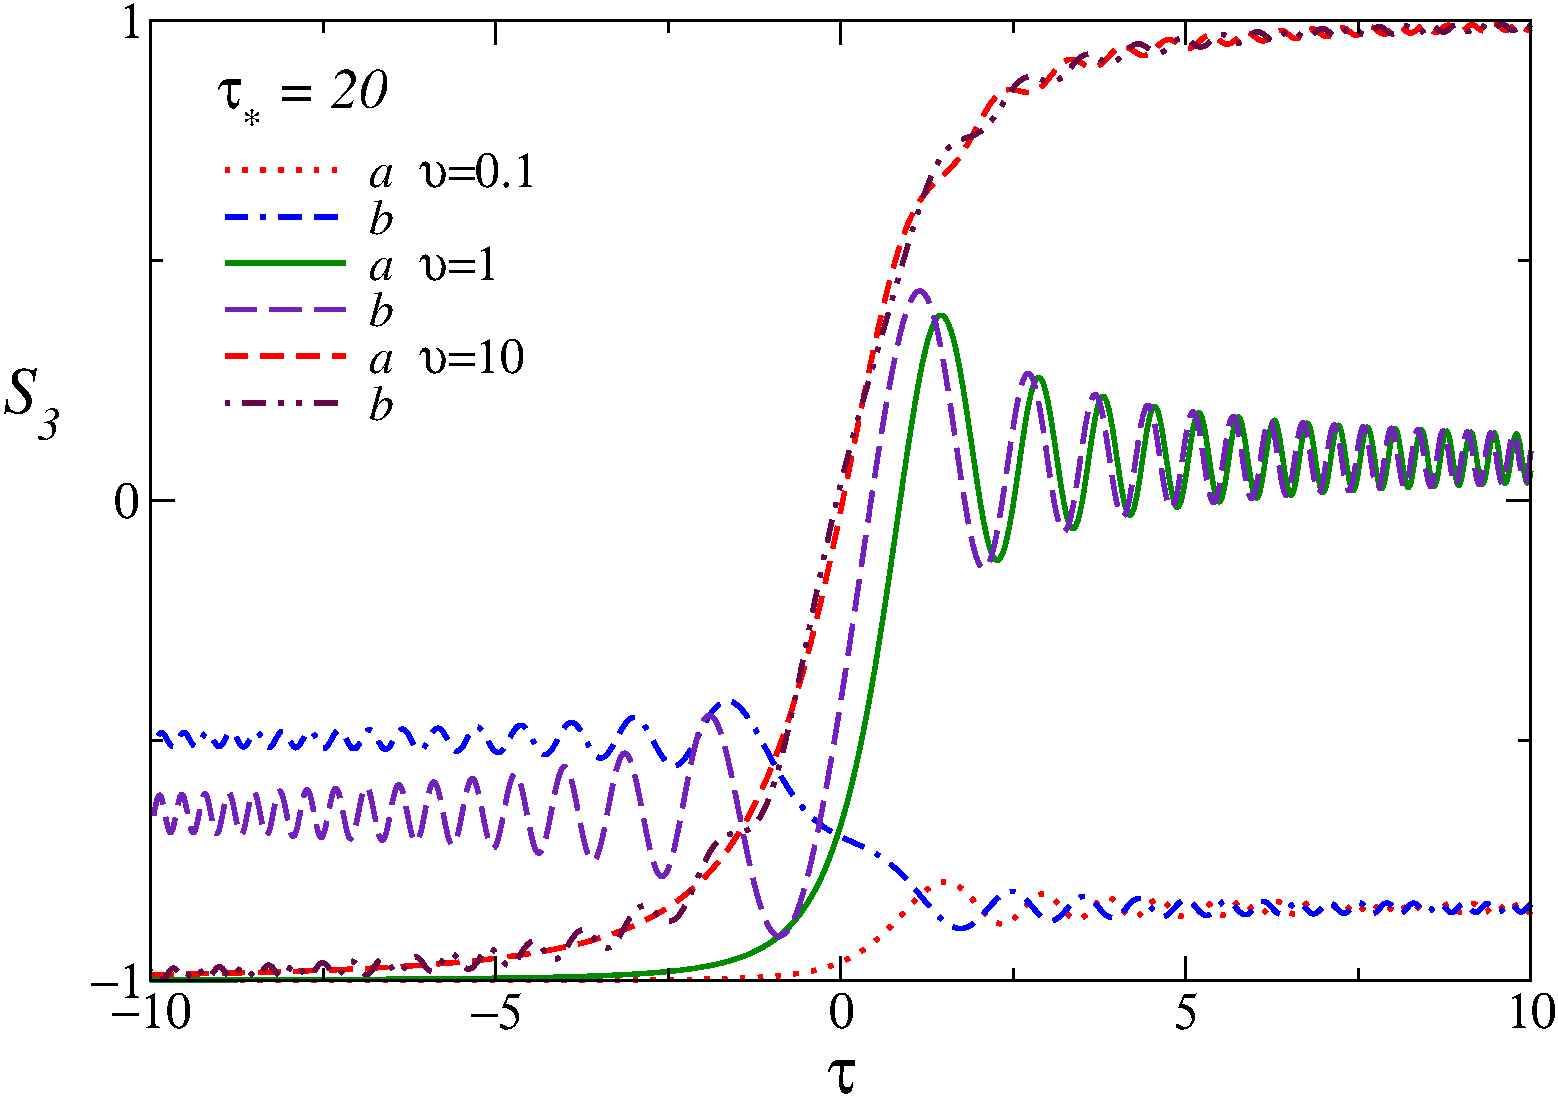
\includegraphics[width=0.55\columnwidth]{imm/mag3taus20.pdf}
      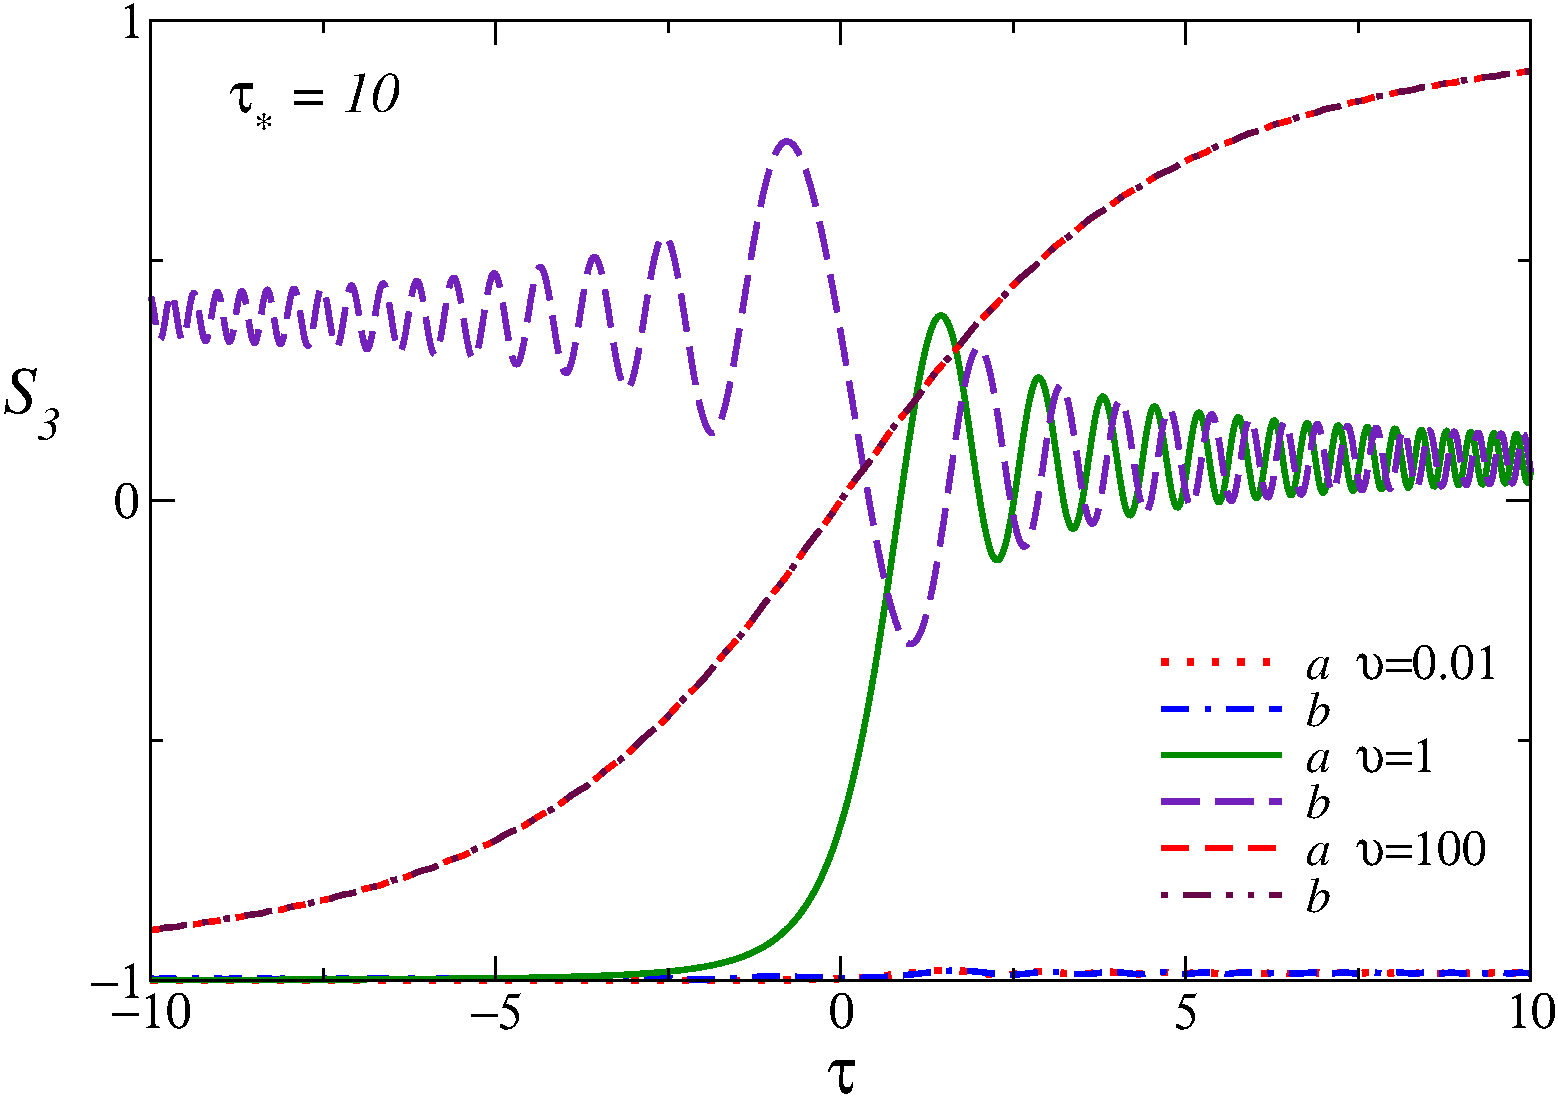
\includegraphics[width=0.55\columnwidth]{imm/mag3taus10.pdf}
  \caption{Evolution of $S_3$ during the protocol, for $\tau_\star=10$
    (bottom) and $\tau_\star=20$ (top), and various values of
    $\upsilon$.}
  \label{lzfigs1}
\end{figure}







Since the variable $\tau$ related to time takes the same values in the
intervals $-t_\star\le t\le t_\star$ and $t_\star\le t\le 3 t_\star$,
we separate  the time dependence in two parts: ($a$) for the first
part where $\beta(t)$ and $\tau$ increases, and ($b$) where $\beta(t)$
and $\tau$ decreases. 
We monitor the dynamic evolution along the protocol defined above by
the expectation values of the operators $\sigma^{(k)}$, i.e.
\begin{eqnarray}
  && S_{3}^{(a/b)}(\upsilon,\tau,\tau_\star) = \langle \Psi(t) |
  \sigma^{(3)} | \Psi(t) \rangle \,,\label{s3def}\\ &&
  S_1^{(a/b)}(\upsilon,\tau,\tau_\star) = \langle \Psi(t) | \sigma^{(1)} |
  \Psi(t) \rangle \,,\label{s1def}
\end{eqnarray}
and the adiabaticity function
\begin{equation}
  A^{(a/b)}(\upsilon,\tau,\tau_\star)
  = |\langle \, \Psi_0, \eta(t) \, | \,
    \Psi(t) \, \rangle|\,.
    \label{addef}
\end{equation}
Note that the adiabatic limit of the evolution
is obtained by sending $\upsilon\to\infty$ keeping fixed
$\kappa$. Therefore,
\begin{equation}
  \lim_{\upsilon\to\infty} A^{(a/b)}(\upsilon, \kappa
  \sqrt{\upsilon}/2, \kappa_\star \sqrt{\upsilon}/2) = 1\,.
  \label{adiablimit}
\end{equation}

Some results for the {\em magnetization} $S_3$ are shown in
Fig.~\ref{lzfigs1} along the first and second branch of the protocol,
for various values of $\upsilon$, $\upsilon=0.01,\,1,\,10000$, and
$\tau_\star=10,\,20$. As expected, the case of large $\upsilon$ the
dynamic tends to be adiabatic, so that the values of $S_3$ along the
two ways tend to superimpose.  In the case of small $\upsilon$ the
dyamic tends to be frozen to the initial condition, moving only
slightly from the initial value. More complex behaviors are observed
for intermediate values of $\upsilon$.

\begin{figure}[!htb]
  \centering
  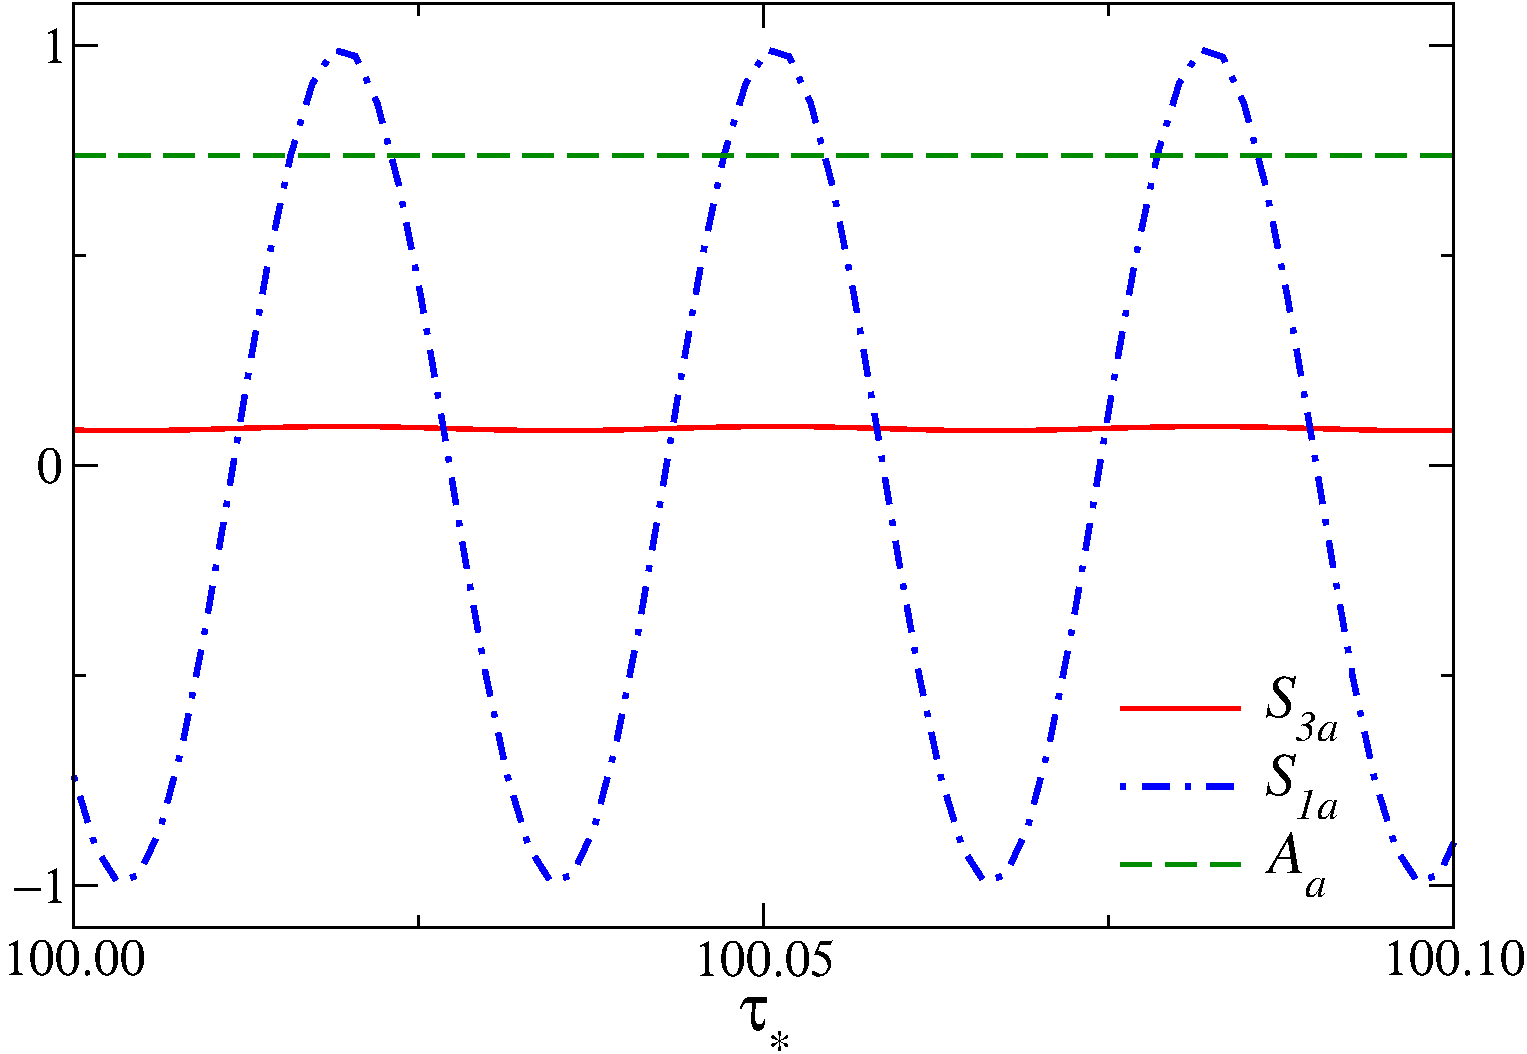
\includegraphics[width=0.55\columnwidth]{imm/oscillationa.pdf}
  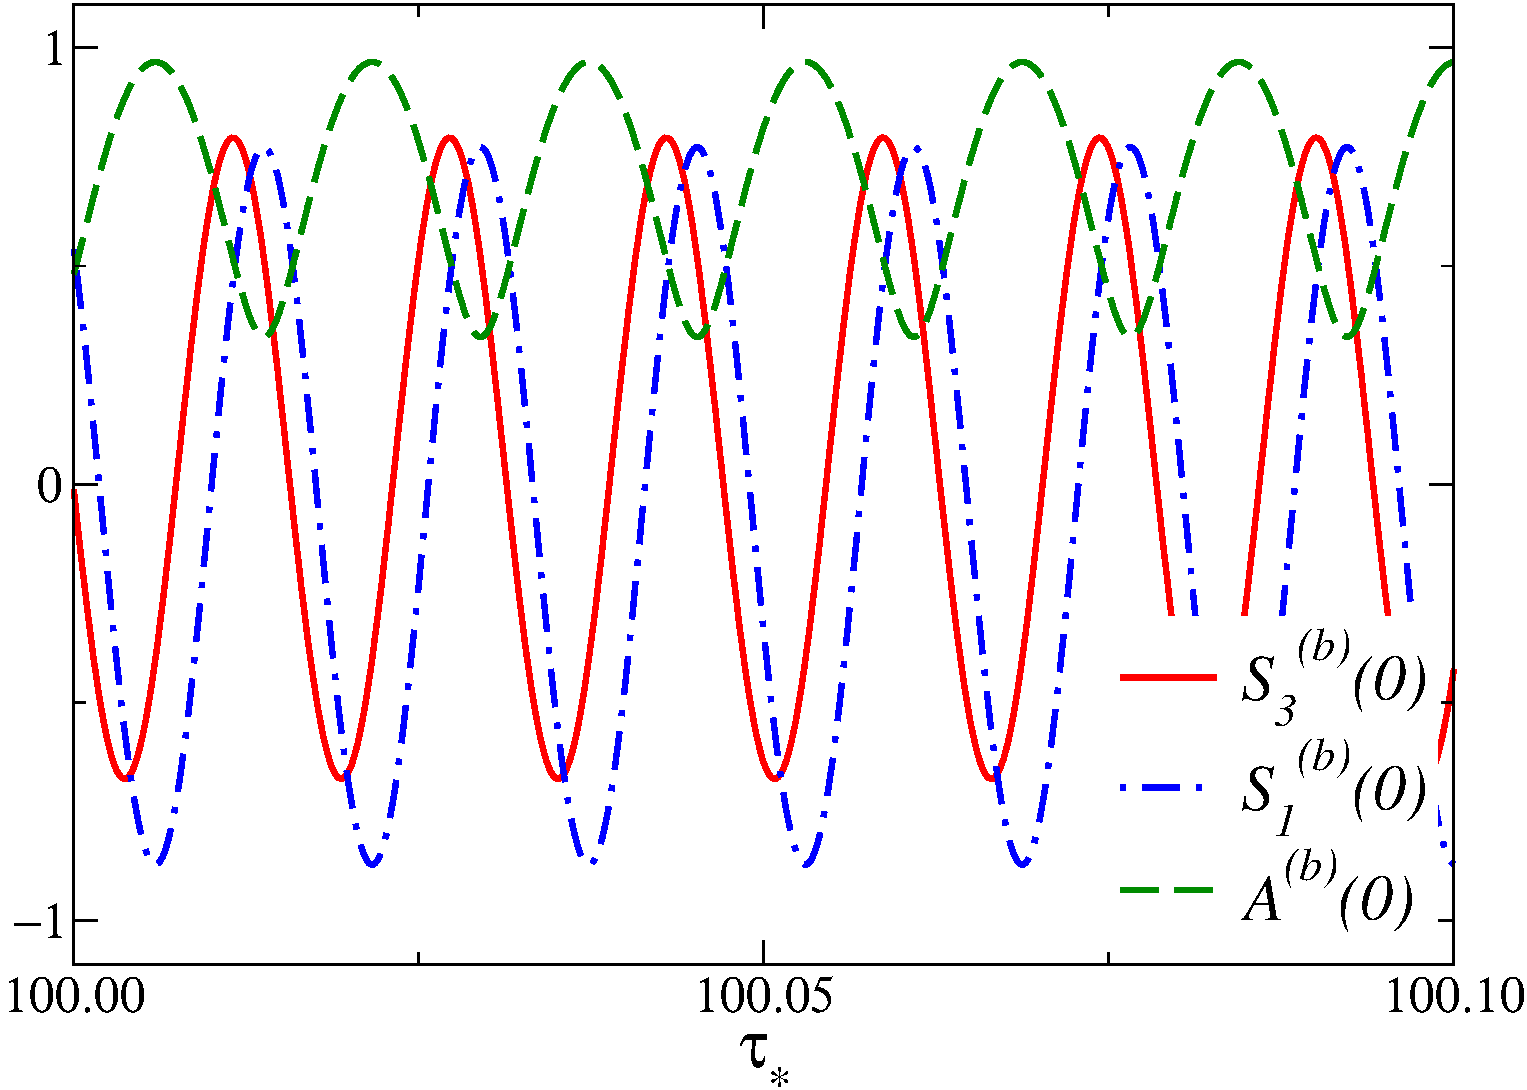
\includegraphics[width=0.55\columnwidth]{imm/oscillationb.pdf}
  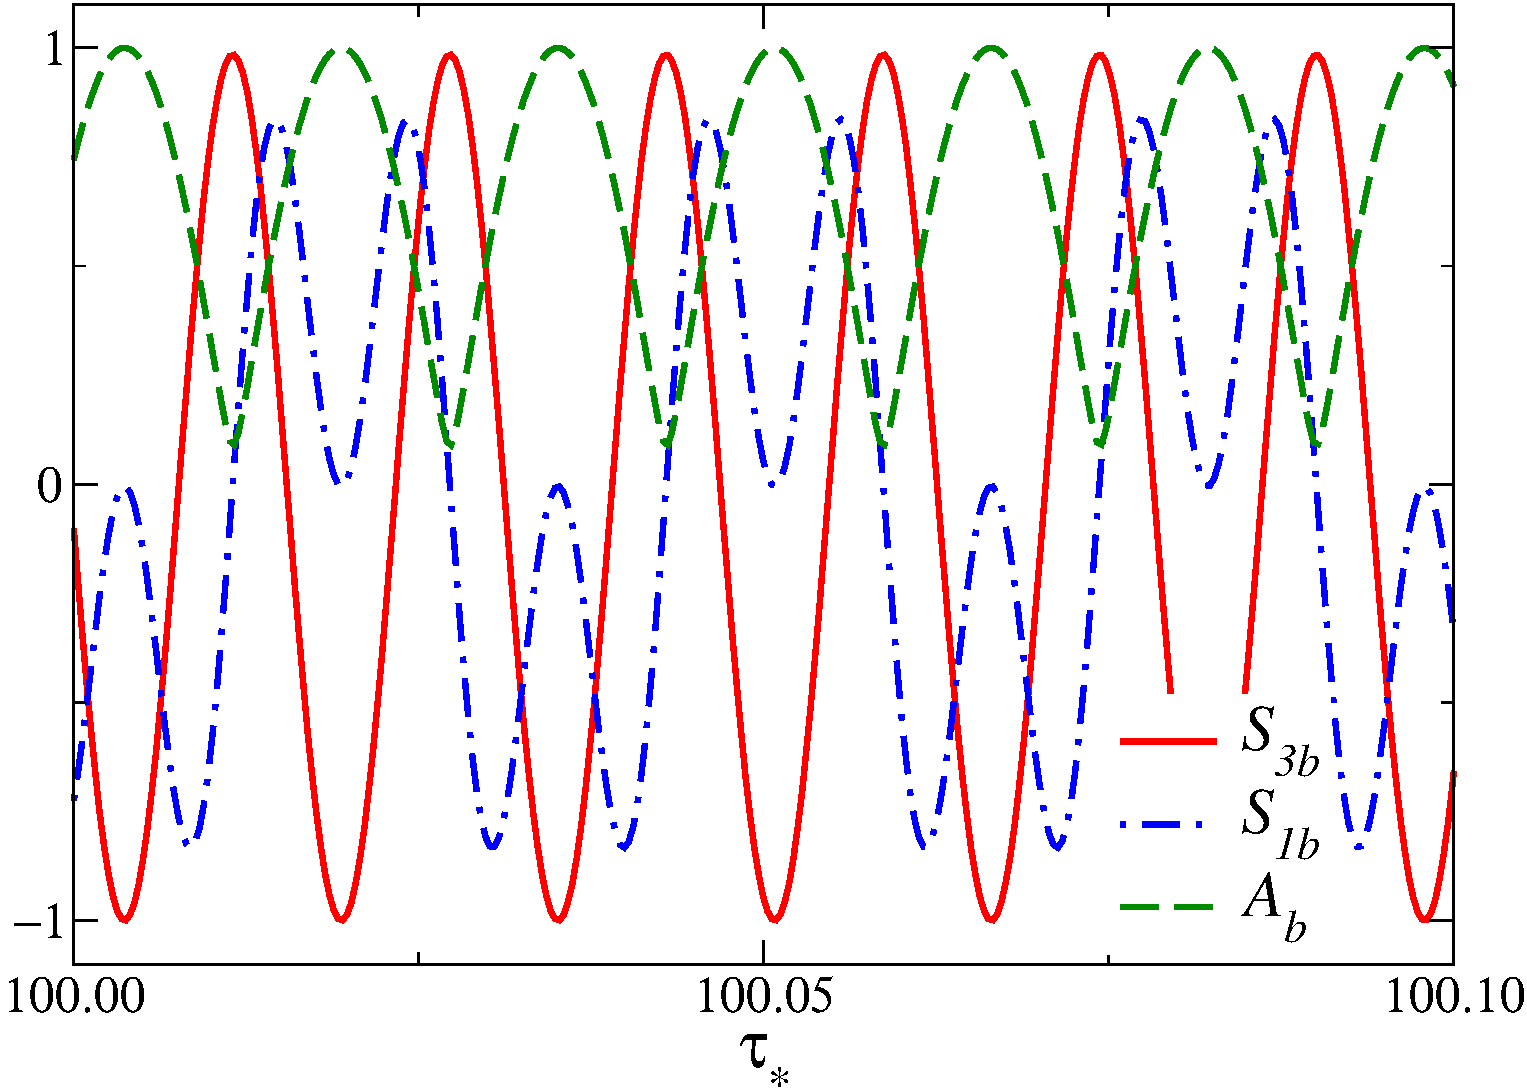
\includegraphics[width=0.55\columnwidth]{imm/oscillationc.pdf}
  \caption{Dependence on $\tau_\star\equiv t_\star/\sqrt{t_s}$ of the
    {\em magnetizations} $S_{1/3}$ and the adiabaticity function $A$
    at the end of the first dynamic branch where $\beta(t)$
    is linearly increasing, and then back along the return way, when
    $\tau=0$ (intermediate) and at the end of the round-trip protocol
    (bottom), for $\upsilon=1$, and $\tau_\star\approx 100$. These
    results show clearly how the oscillations of $S_{1,a}$, and
    therefore of the relative phase of the two functions $\phi_i(t)$
    in Eq.~(\ref{psitbas}), at the end of the first branch are closely
    related to the oscillations of all observables along the return
    way of the round-trip protocol.  }
  \label{lzfigs}
\end{figure}


We now analyze the dynamics of the round-trip protocol in the
large-$\tau_\star$ limit, showing that such limit is problematic for
this problem.  We consider the values of the above observables at the
end of the first and second part of the protocol:
\begin{eqnarray}
 S_{3/1a}(\upsilon,\tau_\star) &=&
  S_{3/1}^{(a)}(\upsilon,\tau_\star,\tau_\star)\,,\label{suddef}\\
  S_{3/1b}(\upsilon,\tau^\star) &=&
  S_{3/1}^{(b)}(\upsilon,-\tau_\star,\tau_\star)\,,\nonumber\\
  A_{a}(\upsilon,\tau_\star)
  &=& A^{(a)}(\upsilon,\tau_\star,\tau_\star)\,,\nonumber\\
 A_{b}(\upsilon,\tau_\star) &=&
  A^{(b)}(\upsilon,-\tau_\star,\tau_\star)\,.\nonumber
\end{eqnarray}

\begin{figure}[!htb]
  \centering
  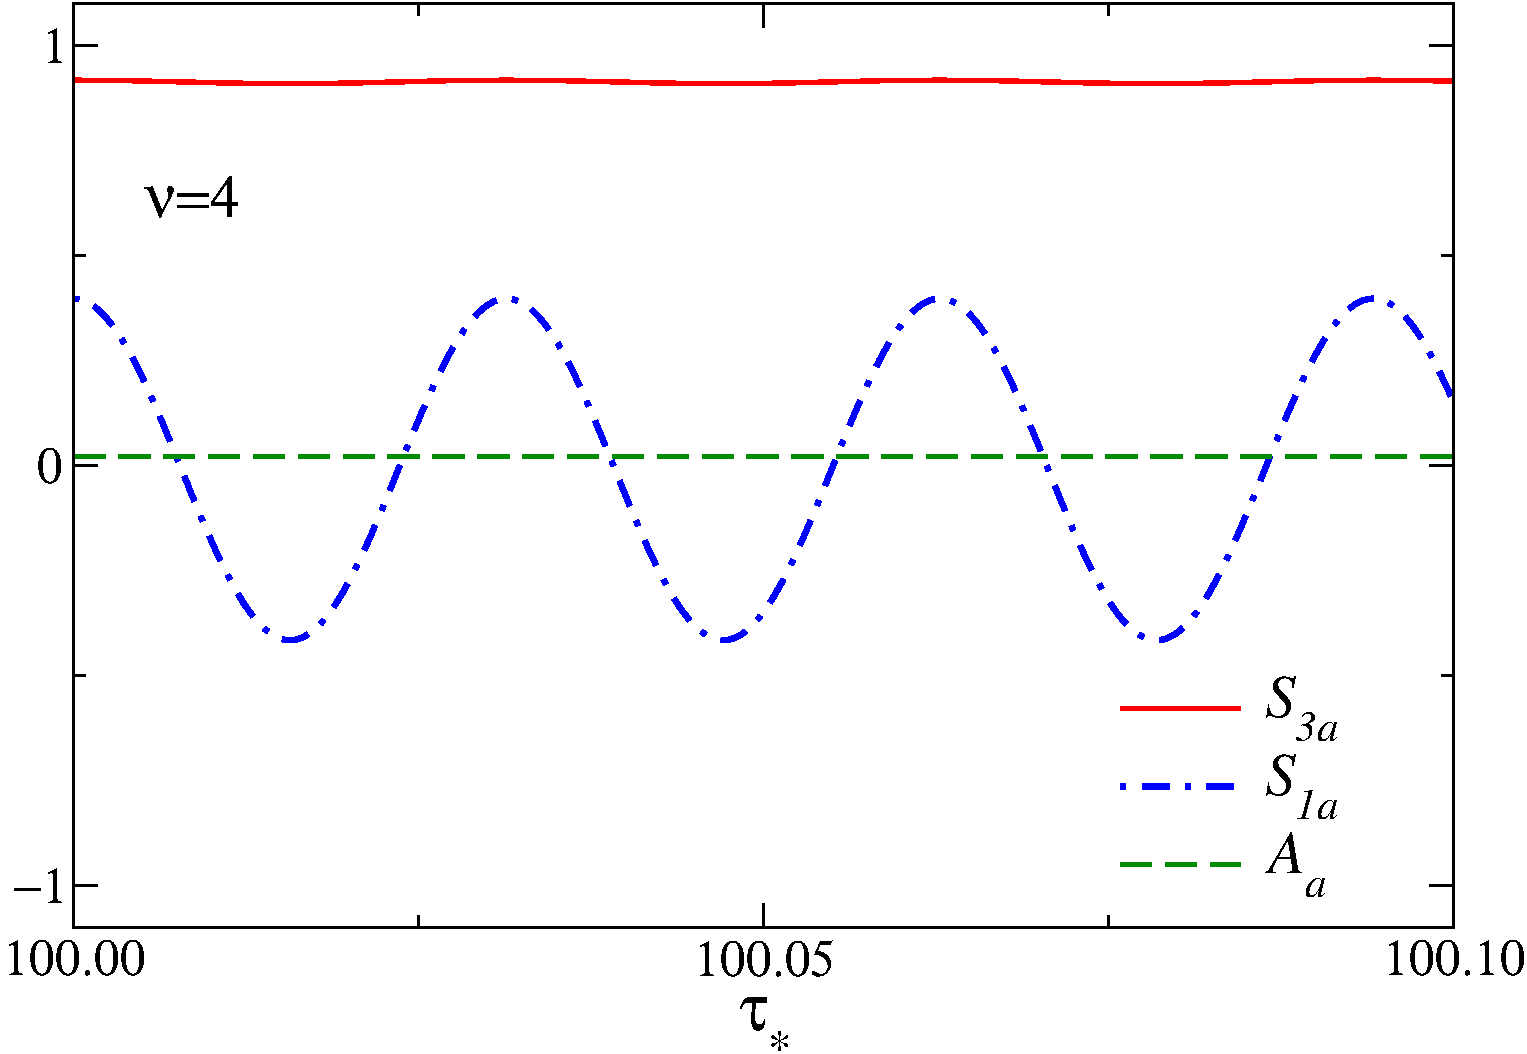
\includegraphics[width=0.55\columnwidth]{imm/oscillation2a.pdf}
  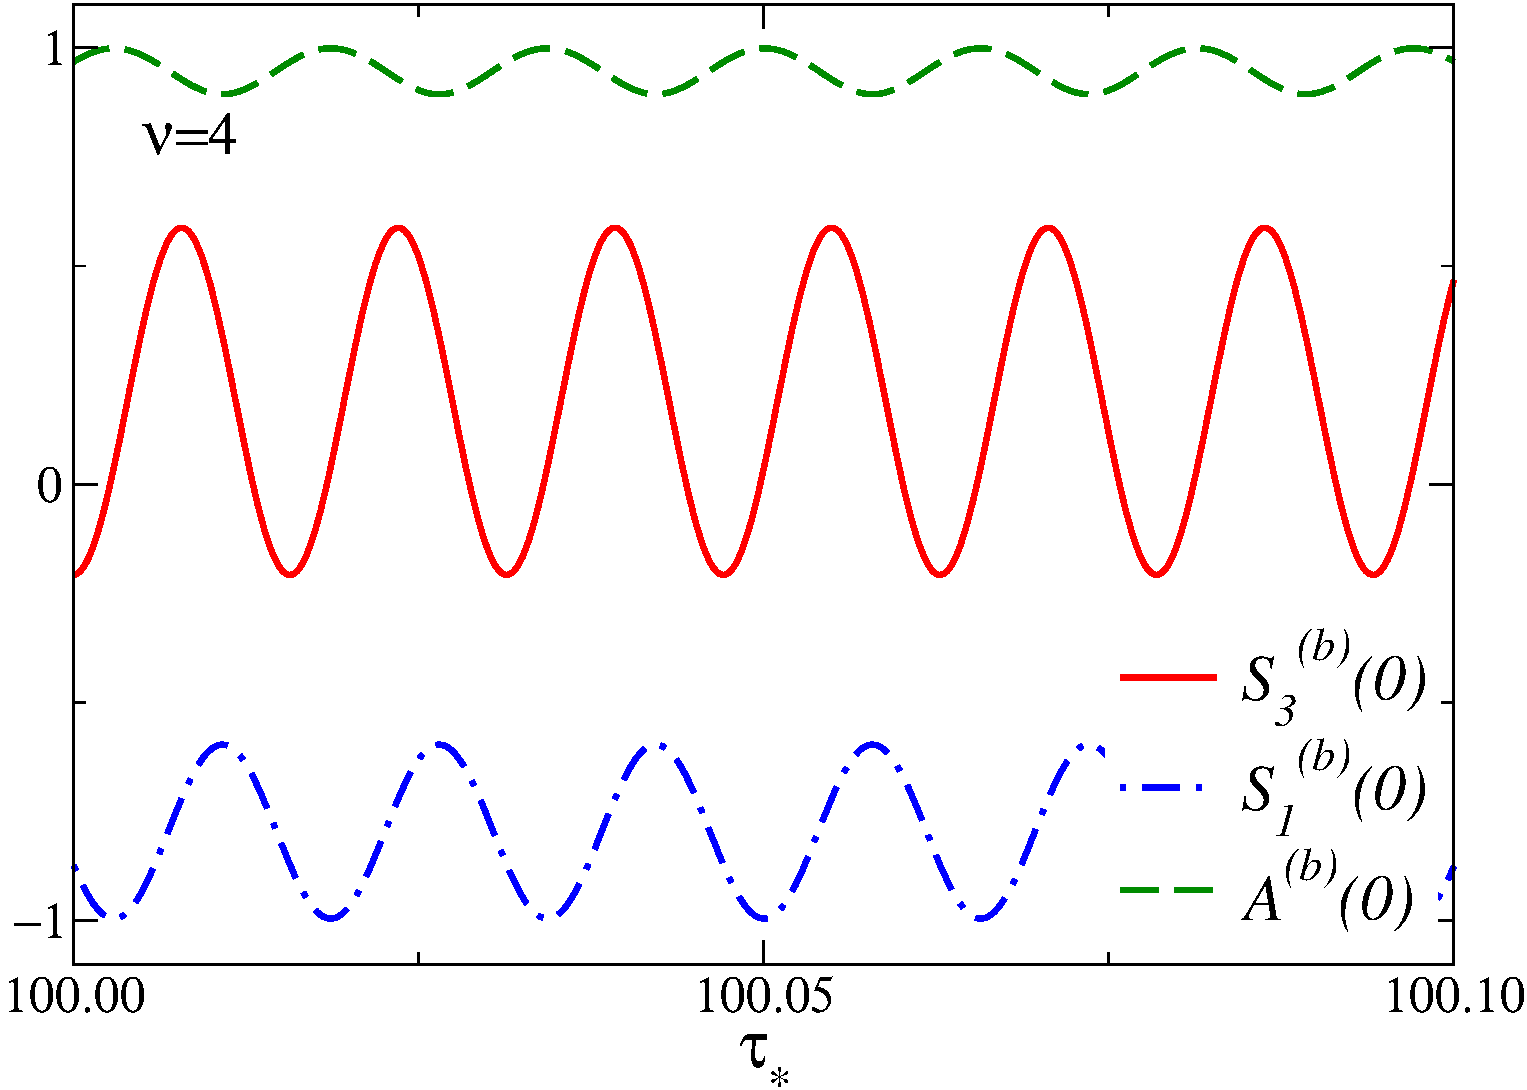
\includegraphics[width=0.55\columnwidth]{imm/oscillation2b.pdf}
  \caption{Dependence on $\tau_\star\equiv t_\star/\sqrt{t_s}$ of the
    {\em magnetizations} $S_{1/3}$ and the adiabaticity function $A$
    at the end of the first dynamic branch where $\beta(t)$
    is linearly increasing, and then back along the return way, when
    $\tau=0$ (bottom), for $\upsilon=4$, and $\tau_\star\approx 100$.}
  \label{lzfigs2}
\end{figure}

\begin{figure}[!htb]
  \centering
  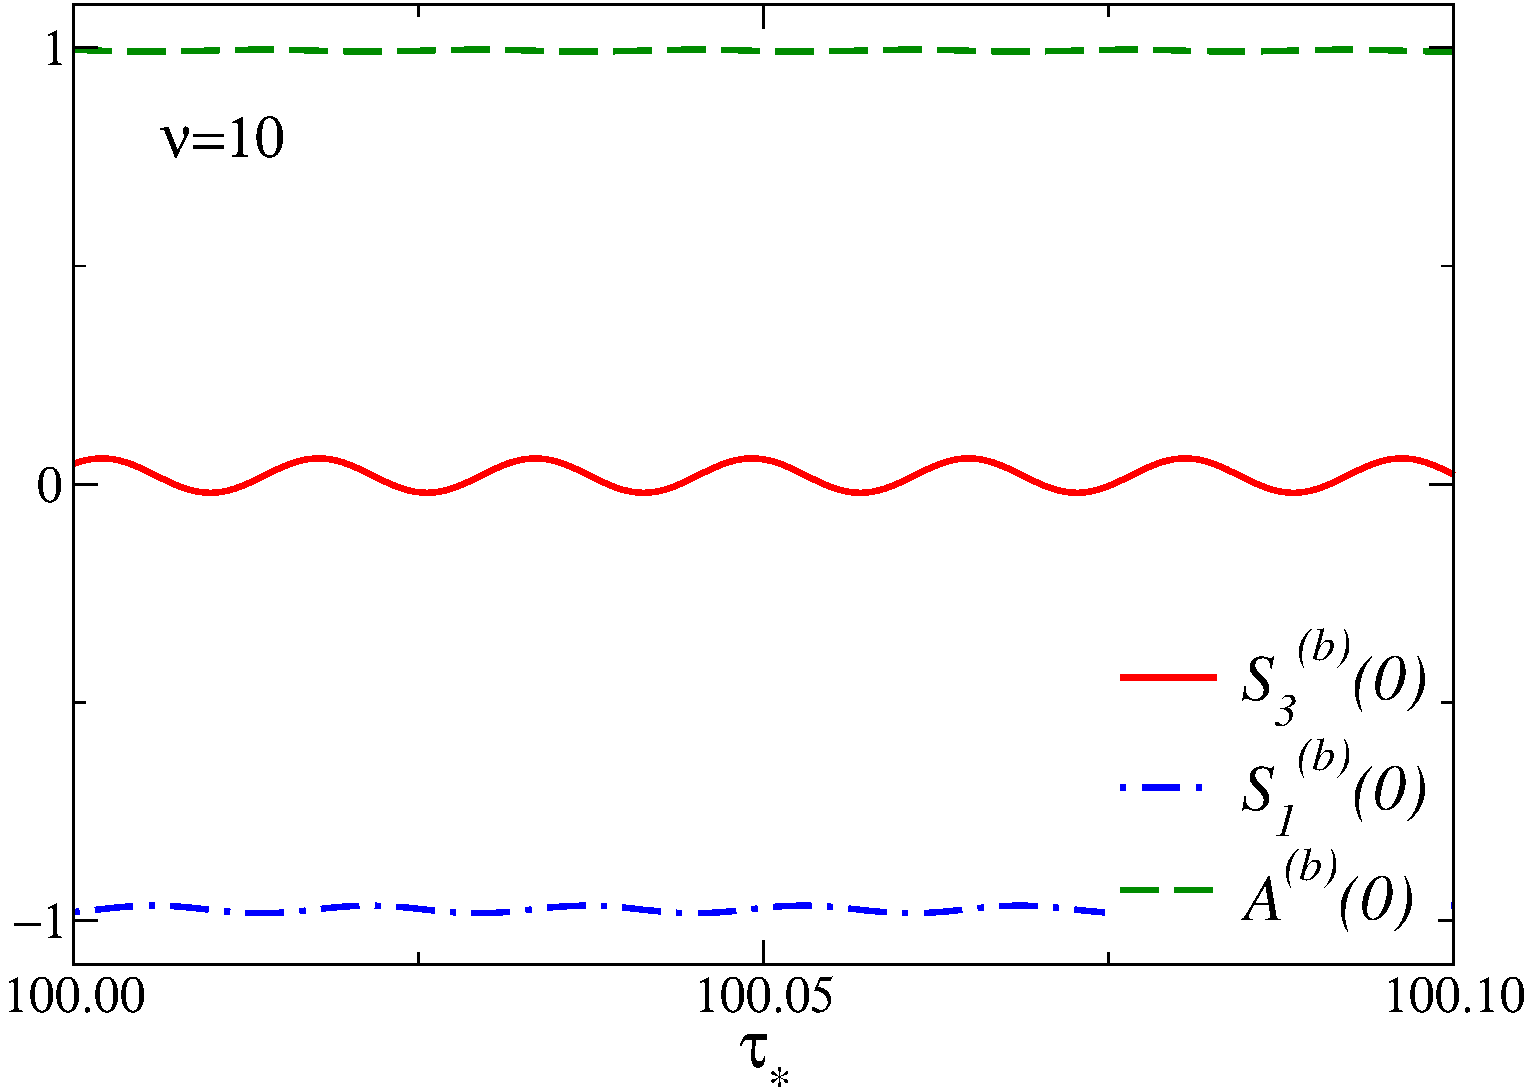
\includegraphics[width=0.55\columnwidth]{imm/oscillation3b.pdf}
  \caption{Dependence on $\tau_\star\equiv t_\star/\sqrt{t_s}$ of the
    {\em magnetizations} $S_{1/3}$ and the adiabaticity function $A$
    along the return way at $\tau=0$, for $\upsilon=10$, and
    $\tau_\star\approx 100$.}
  \label{lzfigs3}
\end{figure}



Some notable limits can be derived for the first branch of the
protocol using the asymptotic behaviors of the parabolic cylinder
functions $D_\nu(x)$~\cite{vitanov1996landau,ISN-22}, corresponding to the
standard LZ problem, see e.g. Refs.~\cite{vitanov1996landau,pelissetto2018out}, such as
\begin{eqnarray}
&&S_{3a}(\upsilon,\tau_\star\to\infty)
= 1 - 2 \,e^{-{\pi \upsilon/4}}\,,\qquad
\label{lzlimit}\\
&&A_a(\upsilon,\tau_\star\to\infty) =
\sqrt{1 - \,e^{-{\pi \upsilon/4}}} \,.\nonumber
\end{eqnarray}
Both $S_{3a}$ and $A_a$ approach their asymptotic behaviors with
oscillating corrections suppressed as $O(\tau_\star^{-1})$. For
example, in the case of the adiabaticity function we find
\begin{eqnarray}
  \Delta A_a &\equiv& 
  A_a(\upsilon,\tau_\star) - A_a(\upsilon,\infty)   \label{asyoscA}\\
&\approx&
  {f(u)\over \tau_\star} \cos[\tau_\star^2 - {u\over 4}\ln\tau_\star +
  g(u)]\,,
\nonumber
\end{eqnarray}
where $f(u)$ and $g(u)$ are time-independent functions of $u$.
Unlike $S_{3a}$ and $A_a$,
the quantity $S_{1a}$ does not show a regular large-$\tau_\star$ limit,
but rapid oscillations with diverging frequency in the large-$\tau^*$
limit.  Indeed, using again the asymptotic behaviors of the parabolic
cylinder functions $D_\nu(x)$~\cite{vitanov1996landau,ISN-22}, the asymptotic
large-$\tau_\star$ behavior of $S_{1,a}$ turns out to be
\begin{eqnarray}
  &&  S_{1a} \approx B(\upsilon)
  %  {\rm Re}\,e^{-i\varphi(\upsilon,\tau^\star)}\,,\qquad
  \cos\varphi(\upsilon,\tau_\star)\,,\qquad
\label{asys1}\\
&& B(\upsilon)=  2 \,e^{-\pi\upsilon/8}\, 
\sqrt{1 - e^{- \pi\upsilon/4}}\; \le 1 \,,\nonumber\\
&& \varphi(\upsilon,\tau_\star) =
\tau_\star^2  + {\upsilon\over 8} \ln(2\tau_\star^2)
- {\rm Arg}\left[\Gamma\left(i{\upsilon\over 8}\right)\right]
+ {3\pi\over 4}\,.
\nonumber
 \end{eqnarray}
In particular, $B(1) = 0.99611...$ and
\begin{equation}
  \varphi(1,\tau_\star)= \tau_\star^2 + {1\over 4} \ln\tau_\star
  + 4.08501...
  \label{var1ttau}
\end{equation}

Unlike $S_{3a}$ and $A_a$ that converge to a large-$\tau_\star$ limit,
the leading behavior of $S_{1a}$ is characterized by rapid
oscillations. Its oscillatory behavior is essentially related to the
relative phase $e^{-i\varphi(u,\tau)}$ of the functions
$\phi_1(u,\tau)$ and $\phi_2(u,\tau)$, cf. Eq.~(\ref{psitbas}).  Note
that oscillations become faster and faster in the large-$\tau^\star$
limit, with a time-dependent frequency $\omega(\tau_\star)$ diverging
as $\omega(\tau_\star)\approx \tau_\star$.  Therefore, unlike $S_{3a}$
and $A_a$ whose oscillations gets suppressed as $1/\tau_\star$
approximately, the quantity $S_{1a}$ does not possess a well defined
large-$\tau_\star$ limit, reflecting the fact that the relative phase
of the $\phi_i$ does not converge in the large-$\tau_\star$ limit.



This fact has dramatic implications for the behavior of the system
along the backward branch, making all quantities rapidly oscillating
at the return point, with a frequency related to that of the relative
phase at the end of the first branch.  This behavior is clearly shown
in Figs.~\ref{lzfigs}, where we report some results for the quantities
defined in Eqs.~(\ref{suddef}), at the end of the first branch and at
the end of the round-trip protocol, and along the return way at
$\tau=0$, at fixed $\upsilon=1$ and as a function of the parameter
$\tau_\star$, for a relatively small interval around
$\tau_\star\approx 100$. As shown by the analogous curves reported in
Figs.~\ref{lzfigs2} and \ref{lzfigs3} for $\nu=4$ and $\nu=10$
respectively, the size of the oscillations depends on the value of
$\nu$, and, as expected, it tends to decreases in the adiabatic limit
when increasing $\nu$.

These results evidentiate the peculiar oscillations in the
large-$\tau_\star$ limit at finite values of $\nu$, which make
predictions on the return behavior practically impossible without an
extreme precision on the control of the parameters of the protocols.

\section{Equilibrium FSS functions}\label{app:eq-FSS-func}
In this appendix, we derive the FSS functions \eqref{eq:eq-scaling-func} for the Ising model \eqref{eq:model} at $h_\perp<1$, in the limit $h_\parallel\to 0^\pm$, $L\to\infty$. As noticed in Refs.~\cite{campostrini2014finite}, the quantum FOT is controlled by the competition of the two lowest energy levels. Therefore, it is possible to write down an effective two-level Hamiltonian by restricting the many-body system to the Hilbert space spanned by the ground state $\ket{\psi_0}$ and the first excited state $\ket{\psi_1}$, obtaining
\be
\hat{H}_\text{eff}=E_0 \hat{{\rm Id}}_{2\times 2} +\frac{1}{2}\left(\Delta(h_\perp,L) \hat\sigma^{(1)} -{\cal E}(h_\perp,h_\parallel,L)\hat\sigma^{(3)}\right),
\ee
where $E_0$ is the ground state energy of the degenerate vacua at $h_\parallel=0$, $L=\infty$. This Hamiltonian is readily diagonalized in the basis
\begin{align}
&\ket{+}=\sin(\frac{\alpha}{2}) \ket{\psi_0} +\cos(\frac{\alpha}{2})\ket{\psi_1}\\
&\ket{-}=\cos(\frac{\alpha}{2}) \ket{\psi_0} -\sin(\frac{\alpha}{2})\ket{\psi_1}
\end{align}
with
\be
\tan(\alpha)=\kappa^{-1}=\frac{\Delta(h_\perp,L)}{{\cal E}(h_\perp,h_\parallel,L)}, \quad 0<\alpha\leq\frac{\pi}{2}.
\ee
It follows that the energy eigenvalues are given by
\be
E_\pm = E_0 \pm \frac{1}{2}\sqrt{{\cal E}^2+\Delta^2}
\ee
and, therefore, the energy gap \eqref{eq:eq-scalingE} reads as
\be
\Delta E(h_\perp,h_\parallel,L)=\Delta(h_\perp,L) \ \sqrt{1+\kappa^2}
\ee
from which one has $f_E(\kappa)=\sqrt{1+\kappa^2}$ (cf~Eq.~\eqref{eq:eq-scaling-func}). The longitudinal magnetization is 
\begin{align}
M(h_\perp,h_\parallel,L)&=M_0(h_\perp) \langle-|\hat\sigma^{(3)}|-\rangle
\nonumber \\[3pt]
&\quad =M_0(h_\perp) \left(\cos^2(\frac{\alpha}{2})-\sin^2(\frac{\alpha}{2})\right),
\end{align}
from which one finds the FSS function (cf.~Eq.~\eqref{eq:eq-scaling-func})
\be
f_M(\kappa)=\cos(\alpha)=\frac{\kappa}{\sqrt{1+\kappa^2}}.
\ee

\section{FSS functions across a FOT}\label{app:OFSS-func}
In this appendix, we focus on the solution of the finite-time LZS problem characterizing the linear driving of the Ising model \eqref{eq:model} across a quantum FOT, see Sec.~\ref{sec:2-lev}. For a better exposition, the case of single and of round-trip passages are treated in different subsections.
\subsection{Single passage}\label{app:LZS-single}
For a single passage through the quantum FOT starting at $\tau_i<0$, the finite-time LZS problem has an analytical solution~--~first derived in Ref.~\cite{vitanov1996landau}. The standard procedure is to decouple the set of equation \eqref{eq:LZS-single} by taking a time derivative. In this way, the differential equation e.g.~for $c_0(\tau,\upsilon)$ takes the form of a Weber differential equation
\be
\frac{d^2}{d\tau^2}c_0(\tau,\upsilon) + (\tau^2+\frac{\upsilon}{4}-i) c_0(\tau,\upsilon)=0,
\ee
which is solved in terms of Parabolic Cylinder functions. It follows that the $2\times 2$ evolution matrix $U(\tau,\tau_i)$ in \eqref{eq:LZS-single} has elements
%\begin{widetext}
\begin{subequations}
\begin{align}
&U_{00}=\frac{\Gamma(1-\frac{i\upsilon}{8})}{\sqrt{2\pi}}\left[\mathscr{D}_{-1+\frac{i\upsilon}{8}}(\sqrt{2}e^{i\frac{3\pi}{4}}\tau_i)\mathscr{D}_{\frac{i\upsilon}{8}}(\sqrt{2}e^{-i\frac{\pi}{4}}\tau) + \mathscr{D}_{-1+\frac{i\upsilon}{8}}(\sqrt{2}e^{-i\frac{\pi}{4}}\tau_i) \mathscr{D}_{\frac{i\upsilon}{8}}(\sqrt{2}e^{i\frac{3\pi}{4}}\tau)\right];\\[4pt]
%%%%%%%%
&U_{01}=\frac{2\Gamma(1-\frac{i\upsilon}{8})}{\sqrt{\pi\upsilon}}e^{i\frac{\pi}{4}}\left[\mathscr{D}_{\frac{i\upsilon}{8}}(\sqrt{2}e^{-i\frac{\pi}{4}}\tau_i)\mathscr{D}_{\frac{i\upsilon}{8}}(\sqrt{2}e^{i\frac{3\pi}{4}}\tau) - \mathscr{D}_{\frac{i\upsilon}{8}}(\sqrt{2}e^{i\frac{3\pi}{4}}\tau_i) \mathscr{D}_{\frac{i\upsilon}{8}}(\sqrt{2}e^{-i\frac{\pi}{4}}\tau)\right],
\end{align}
\end{subequations}
with $U_{10}=-U_{01}^*$ and $U_{11}=U_{00}^*$, $\Gamma(z)$ is the Euler Gamma function.\\
%\end{widetext}
In the limit $|\tau_i|\gg 1$, these expressions can be simplified using known relations for $\mathscr{D}_\nu(z)$, reading as
\begin{subequations}\label{eq:U-large}
\begin{align}
&U_{00}(|\tau_i|\gg 1)\simeq e^{i\Phi(\tau_i,\upsilon)} e^{-\frac{\pi\upsilon}{32}} \mathscr{D}_{\frac{i\upsilon}{8}}(\sqrt{2}e^{i\frac{3\pi}{4}}\tau);\\[4pt]
%%%%%%%%
&U_{10}(|\tau_i|\gg 1)\simeq e^{i\Phi(\tau_i,\upsilon)}\sqrt{\frac{\upsilon}{8}} e^{-i\frac{\pi}{4}} e^{-\frac{\pi\upsilon}{32}} \mathscr{D}_{-1+\frac{i\upsilon}{8}}(\sqrt{2}e^{i\frac{3\pi}{4}}\tau),
\end{align}
\end{subequations}
and the dependence on the initial condition $\tau_i$ drops out everywhere but in the phase
\be\label{eq:phase}
\Phi(q,\upsilon)=-q^2-\frac{\upsilon}{4}\log(\sqrt{2}|q|).
\ee
One can then easily obtain the expressions in Eqs.~\eqref{eq:OFSS-func-M-single}-\eqref{eq:OFSS-func-A-single} for the FSS functions. The latter do not show any dependence on the initial condition $\tau_i$. It is interesting to note that by taking the limit $\tau\to\infty$ in Eq.~\eqref{eq:OFSS-func-M-single}, one obtains the Landau-Zener prediction for the defects abundance
\be
{\cal F}_M(\tau\to\infty,\upsilon)=1-2e^{-\frac{\pi\upsilon}{4}},
\ee
in agreement with standard Kibble-Zurek arguments \cite{dziarmaga2010dynamics}.
\subsection{Round trip}
With a similar strategy, it is possible to extend the solution of Appendix~\ref{app:LZS-single} to the round-trip protocol, by solving the two-level problem in the interval $t\in[t_f, 2t_f+|t_i|]$. Denoting with
\be
x=\frac{t_f+|t_i|-t}{\sqrt{u}},
\ee
one finds the following elements of the $2\times 2$ evolution matrix $\tilde{U}(\tau,\tau_f)$ in \eqref{eq:LZS-round-trip}:
%\begin{widetext}
\begin{subequations}
\begin{align}
&\tilde{U}_{00}=\frac{\Gamma(1-\frac{i\upsilon}{8})}{\sqrt{2\pi}}\left[\mathscr{D}_{\frac{i\upsilon}{8}}(\sqrt{2}e^{i\frac{3\pi}{4}}|\tau_i|)\mathscr{D}_{-1+\frac{i\upsilon}{8}}(\sqrt{2}e^{-i\frac{\pi}{4}}x) + \mathscr{D}_{\frac{i\upsilon}{8}}(\sqrt{2}e^{-i\frac{\pi}{4}}|\tau_i|) \mathscr{D}_{-1+\frac{i\upsilon}{8}}(\sqrt{2}e^{i\frac{3\pi}{4}}x)\right];\\[4pt]
%%%%%%%%
&\tilde{U}_{10}=\frac{2\Gamma(1-\frac{i\upsilon}{8})}{\sqrt{\pi\upsilon}}e^{i\frac{\pi}{4}}\left[\mathscr{D}_{\frac{i\upsilon}{8}}(\sqrt{2}e^{i\frac{3\pi}{4}}|\tau_i|)\mathscr{D}_{\frac{i\upsilon}{8}}(\sqrt{2}e^{-i\frac{\pi}{4}}x) - \mathscr{D}_{\frac{i\upsilon}{8}}(\sqrt{2}e^{-i\frac{\pi}{4}}|\tau_i|) \mathscr{D}_{\frac{i\upsilon}{8}}(\sqrt{2}e^{i\frac{3\pi}{4}}x)\right],
\end{align}
\end{subequations}
with $\tilde{U}_{01}=-\tilde{U}_{10}^*$ and $\tilde{U}_{11}=\tilde{U}_{00}^*$. \\
%\end{widetext}
Similarly to the previous case, these expressions simplify in the limit $|\tau_i|\gg 1$:
\begin{subequations}
\begin{align}
&\tilde{U}_{11}(|\tau_i|\gg 1)\simeq e^{i\Phi(\tau_i,\upsilon)} e^{-\frac{\pi\upsilon}{32}} \mathscr{D}_{\frac{i\upsilon}{8}}(\sqrt{2}e^{-i\frac{\pi}{4}}x);\\[4pt]
%%%%%%%%
&\tilde{U}_{01}(|\tau_i|\gg 1)\simeq e^{i\Phi(\tau_i,\upsilon)}\sqrt{\frac{\upsilon}{8}} e^{-i\frac{\pi}{4}} e^{-\frac{\pi\upsilon}{32}} \mathscr{D}_{-1+\frac{i\upsilon}{8}}(\sqrt{2}e^{-i\frac{\pi}{4}}x).
\end{align}
\end{subequations}
From these equations (together with~\eqref{eq:U-large}), one finds
\begin{subequations}
\be\begin{split}\label{eq:coef0-round}
&c_0=e^{-\frac{\pi\upsilon}{16}}\Big\{\mathscr{D}_{\frac{i\upsilon}{8}}(\sqrt{2}e^{i\frac{3\pi}{4}}\tau_f)[\mathscr{D}_{\frac{i\upsilon}{8}}(\sqrt{2}e^{-i\frac{\pi}{4}}x)]^*\\[3pt]
&\qquad- \frac{i\upsilon}{8} e^{2i\Phi(\tau_i,\upsilon)}  \mathscr{D}_{-1+\frac{i\upsilon}{8}}(\sqrt{2}e^{i\frac{3\pi}{4}}\tau_f) \mathscr{D}_{-1+\frac{i\upsilon}{8}}(\sqrt{2}e^{-i\frac{\pi}{4}}x)\Big\};
\end{split}\ee
%%%%%%%%%%%%%%%%%%%%
\be\begin{split}\label{eq:coef1-round}
&c_1=e^{-\frac{\pi\upsilon}{16}} \sqrt{\frac{\upsilon}{8}} e^{i\frac{\pi}{4}}\Big\{-\mathscr{D}_{\frac{i\upsilon}{8}}(\sqrt{2}e^{i\frac{3\pi}{4}}\tau_f)[\mathscr{D}_{-1+\frac{i\upsilon}{8}}(\sqrt{2}e^{-i\frac{\pi}{4}}x)]^*\\[3pt]
&\quad-i e^{2i\Phi(\tau_i,\upsilon)}  \mathscr{D}_{-1+\frac{i\upsilon}{8}}(\sqrt{2}e^{i\frac{3\pi}{4}}\tau_f) \mathscr{D}_{\frac{i\upsilon}{8}}(\sqrt{2}e^{-i\frac{\pi}{4}}x)\Big\},
\end{split}\ee
\end{subequations}
and determines the FSS functions as detailed in the main text. \\

Notice that the coefficients \eqref{eq:coef0-round}-\eqref{eq:coef1-round} (hence the FSS functions) keep a non-trivial dependence on the initial condition $\tau_i$ during the non-equilibrium dynamics via the phase \eqref{eq:phase}. This is not surprising given that $x_i\equiv |\tau_i|$ is the time at which the ramp is inverted after the first passage across the quantum FOT. At this time, the system is far from equilibrium and hence unable to wash out the memory on its initial (non-equilibrium) condition before being driven across the quantum FOT for the second time.

\chapter{Liouvillian gap}
\label{appa}


\section{Steady-state solution and $\Delta_\lambda$ for $b=1$.}
\label{sec_steadystate}
In this appendix, we discuss the spectrum of the Liouville superoperator $\mathcal{L}[\rho]$ appearing in Eq.~\eqref{eqlindblad} for the case $b=1$. In particular, we focus on the Liouvillian gap $\Delta_\lambda$ and the steady-state solution. The study is dramatically simplified after we move to the momentum basis. To this end, let us first review the unitary Kitaev ring in momentum space in the absence of dissipation. 

We define the Fourier transform of the operator $\hat{c}_x$ as~\cite{NRV-2019-competingdissipativeandcoherent}
\begin{equation}
    \hat{c}_x=\frac{e^{-i\pi/4}}{\sqrt{L}}\sum_{k}e^{ikx}\hat{c}_k\,, \quad k=\bigg\{\pm\frac{(2n-1)\pi}{L}\bigg\}\,,
\end{equation}
where the momenta are induced by the boundary conditions used and $n=1,\dots, L/2$. To simplify the discussion, we only consider even lattice sizes, so that $L/2$ is always an integer number. For each mode $k>0$, we can choose an ordered Hilbert-space basis of the form $\{\ket{0_k},\ket{1_k},\ket{1_{-k}}, \ket{1_{k,-k}}\}$, where the hamiltonian is $\hat{H}=\sum_{k>0}\hat{H}_k$ with
\begin{equation}
    \hat{H}_k=\begin{pmatrix}
    0 & 0 & 0 & 2\abs{\sin k}\\
    0 & -2f_k(\mu) & 0 & 0\\
    0& 0 & -2f_k(\mu)&0\\
    2\abs{\sin k}& 0& 0& -4f_k(\mu)\\
    \end{pmatrix}\,,
    \label{eq_app_Hk_b1}
\end{equation}
and $f_k=\mu/2+\cos k$~\cite{NRV-2019-competingdissipativeandcoherent, P-2008-thirdquantization}. The full Hilbert space $\mathcal{H}$ decomposes naturally into the direct product of $n$ distinct $4$-dimensional subspaces. We take advantage of this transformation, which allows us to trade the exponential complexity of the starting problem with a polynomial one. 

The same change of basis simplifies the study even in the presence of dissipation. If we consider the eigenvalue problem related to Eq.~\eqref{eqlindblad} in momentum space, we get
\begin{equation}
\mathcal{L}[\rho]=\sum_{k>0}\mathcal{L}_k[\rho_k]\,,\quad \mathcal{L}_k[\rho_{k}]=\beta^{(j)}_{k}\rho^{(j)}_{k}\,,
\label{eq_mathcal_L_k}
\end{equation}
where $\rho=\bigotimes_{k>0}\rho_k$ and the superoperator $\mathcal{L}_k$ reads as
\begin{equation}
\begin{aligned}
        \mathcal{L}_k[\rho_k]=&-i[H_k,\rho_k]+w\hat{c}_{k}\rho_k\hat{c}_{k}^{\dagger}-\frac{w}{2}\{c^\dagger_{k}\hat{c}_{k}, \rho_k\}\\
        &+w\hat{c}_{-k}\rho_k\hat{c}_{-k}^{\dagger}-\frac{w}{2}\{c^\dagger_{-k}\hat{c}_{-k}, \rho_k\}\,.
\end{aligned}
\label{eq_app_def_mathcalL_momentum}
\end{equation}
In eq.~\eqref{eq_mathcal_L_k}, the complex number $\beta^{(j)}_{k}\in\mathbb{C}$ denotes the $j$-th eigenvalue associated with the $k$-th Hilbert space, so that $\lambda_r$ are the eigenvalues of $\mathcal{L}$ that are fully specified by $\lambda_r=\sum_k\beta_k^{(a_k)}$ with $a_k=1,\dots,16$. Within each momentum sector, the $16$ eigenvalues $\beta^{(j)}_k$ are explicitly given by
\begin{equation}
    \beta^{(j)}_k=
    \begin{cases}
        0\\
        -w \quad &\text{deg. 4}\\
        -w/2\pm\sqrt{-4-\mu^2-4\mu\cos{k}}\quad &\text{deg. 2}\\
        -w\pm2\sqrt{-4-\mu^2-4\mu\cos{k}}\\
        -3w/2\pm\sqrt{-4-\mu^2-4\mu\cos{k}}\quad &\text{deg. 2}\\   
        -2w\,,
    \end{cases}
\end{equation}
where on the right side we indicate the degeneracy of each eigenvalue. It is now simple to show that the Liouville gap is always equal to 
\begin{equation}
\Delta_\lambda=\frac{w}{2}\,,
\label{eq_liouville_gap_w_2}
\end{equation}
independently of the chemical potential $\mu$ considered. The NESS is the only matrix $\rho^{(0)}$ surviving at asymptotically large times; it satisfies $\mathcal{L}_k[\rho^{(0)}_k]=0$ for all $k>0$. We remark that the existence and uniqueness of a steady-state solution, in general terms, cannot be taken for granted~\cite{N-2019-uniquenesslindblad}. Nonetheless, we were able to find a closed-form expression for this state within each Hilbert domain $\mathcal{H}_{k}$
\begin{equation}
\scriptsize{
\rho^{(0)}_k=
\begin{pmatrix}
    1-\frac{3(1-\cos(2k))}{2g_k(\mu,w)} & 0 &0&
    \frac{|\sin k|(2\mu+i w+4\cos k)}{2g_k(\mu,w)}\\
    0 & \frac{\sin^2k}{g_k(\mu,w)} &0&0\\
    0 & 0&\frac{\sin^2k}{g_k(\mu,w)} &0\\
        \frac{|\sin k|(2\mu-i w+4\cos k)}{2g_k(\mu,w)} & 0&0&\frac{\sin^2k}{g_k(\mu,w)}
\end{pmatrix}
}
\end{equation}
where $g_k(\mu,w)=4+\mu^2 + w^2/4 + 4\mu \cos 
k$. Even if the system is coupled with particle-decay operators that continuously remove particles from the ring, the NESS can exhibit a non-vanishing density of fermions—the total number of particles is not preserved by $\hat{H}$. For instance, the average number of particles per site in the asymptotic limit $t\to+\infty$ is
\begin{equation}
    \frac{1}{L}\sum_x\langle\hat{n}_x\rangle=\frac{4}{L}\sum_{n=1}^{L/2}\frac{\sin^2\big[\frac{(2n-1)\pi}{L}\big]}{4+\mu^2+\frac{w^2}{4}+4\mu\cos[\frac{(2n-1)\pi}{L}]}\,.
\end{equation}
We verified numerically the above equation. 

\section{Simulation techniques}
\label{sec_app_simulation}
In this Appendix, we summarize the numerical techniques employed for the real-time evolution of the Kitaev ring in Eq.~\eqref{dissipator} and the determination of the gap $\Delta_\lambda$~\cite{P-2008-thirdquantization}. We also review the Kitaev model investigated in this thesis in momentum space for $b\geq1$.

\subsection{Time evolution of two-point functions (coordinate space)}
\label{sec_app_coordinate_space}

The algorithmic details related to the real-time evolution of correlation functions are thoroughly explained in Refs.~\cite{NRV-2019-competingdissipativeandcoherent, TV-2021-dissipativeboundaries}. We generalize these techniques to the dissipation mechanism described by Eq.~\eqref{eqlindblad}. We adopt these numerical techniques every time the number of local dissipators $n$ is fixed. Essentially, we find a closed system of coupled differential equations allowing us to describe the time evolution of the two-point functions $C(x, y, t)=C_{x,y}$ and $P(x, y, t)=P_{x,y}$ defined in Eq.~\eqref{eq_def_two_point_functions_C_P}. Differentiating these observables with respect to time, we obtain the following differential equations
\begin{eqnarray}
&&  \frac{d}{dt}\,{C}_{x,y} = i\,({C}_{x,y+1} -
  {C}_{x-1,y} + {C}_{x,y-1} - {C}_{x+1,y})
  \qquad \label{eqscxy}\\
&&\quad -i \, ({P}_{y,x-1}^\dagger
  - {P}_{y,x+1}^\dagger - {P}_{x,y-1} + {P}_{x,y+1})
  \nonumber \\
  & &  \quad
  - \frac{w}{2} \sum_{\overset{j=1}{\text{(mod b)}}}^n \,( \delta_{j,y}\,
  {C}_{x,j} + \delta_{j,x}\, {C}_{j,y} 
+\delta_{j,y}\, {C}_{x,j} + \delta _{1,j}\,
  {C}_{j,y}) \nonumber\\
&&\quad  \,,\nonumber\\
&&\frac{d}{dt}\,{P}_{x,y} = -i\,({P}_{x,y+1} +
    {P}_{x+1,y}+ {P}_{x,y-1} + {P}_{x-1,y})
    \nonumber\\
 && \quad -
i\,( {C}_{x,y-1} -
{C}_{y,x-1} - {C}_{x,y+1} 
+ {C}_{y,x+1}) \nonumber \\
 && \quad -
i\,(\delta_{x-1,y} - \delta_{x+1,y})
- 2\,i\,\mu \,{P}_{x,y} \nonumber \\
&&\quad - \frac{w}{2} \sum_{\overset{j=1}{\text{(mod b)}}}^n\,(\delta_{j,y}\,{P}_{x,j} +
\delta_{j,x}\,{P}_{j,y}+ \delta _{j,y}\,{P}_{x,j}
+ \delta_{j,x}\,{P}_{j,y}) \,.  
\nonumber
\end{eqnarray}
We then use standard $4^{\text{th}}$-order Runge-Kutta techniques to solve this system, using the initial conditions given by
\begin{align}
    C_{x,y}(0)&={\rm Tr}[\rho(0)(\hat{c}^\dagger_x\hat{c}_y+\hat{c}^\dagger_y\hat{c}_x)]\\
    P_{x,y}(0)&={\rm Tr}[\rho(0)(\hat{c}^\dagger_x\hat{c}^\dagger_y+\hat{c}_y\hat{c}_x)]\,.
    \label{eq_operators_CP_in_appendix}
\end{align}

\subsection{Time evolution for $b\geq1$ (momentum space)}
\label{sec_app_momentum_space}

Following the quench protocol outlined in Sec.~\ref{sec_observables}, we first set the starting density matrix $\rho(0)$ to the ground state of $\hat{H}$ from Eq.~\eqref{eq_app_Hk_b1}. In particular, the mixture $\rho(0)$ can be rewritten in terms of the reduced density matrices defined within each $k$-sector $\rho_k(0)=\ket{\Omega_k}\bra{\Omega_k}$ as
\begin{equation}
    \rho(0)=\bigotimes_{k>0}\rho_k(0)\,.
\end{equation}
For $t>0$, unfortunately, $\rho_k(t)$ does not remain inside the same $k$-sector as $\rho_k(0)$ (unless $b=1$), and we are forced to study the time evolution of $\rho_k(t)$ in larger domains. For this reason, we define $n/2$ orthogonal Hilbert subspaces $\mathcal{H}_{k_a}$, whose dimension is $4^b$, generated by
\begin{equation}
\mathcal{H}_{k_a}=\text{span}\bigotimes_{m=1}^b\{\ket{0_{k_{a}^m}}, \ket{1_{k_{a}^m}}, \ket{1_{-k_{a}^m}}, \ket{1_{k_{a}^m,-k_{a}^m}}\}\,,
\end{equation}
where $k^m_a\equiv k_a+2\pi m/b$ and $k_a=\pi(2a-1)/L$ with $a=1,\dots,n/2$. We then express $\rho(t)$ as $\rho=\bigotimes_{a=1}^{n/2}\rho_{k_a}$, where $\rho_{k_a}$ is a reduced density matrix living entirely in $\mathcal{H}_{k_a}$. The time evolution of each $\rho_{k_a}$ is controlled by a self-contained Lindblad equation
\begin{equation}
    \frac{d\rho_{k_a}}{dt}=-i[\hat{H}_{k_a},\rho_{k_a}]+w\mathbb{D}[\rho_{k_a}]\,,
\end{equation}
where $\hat{H}_{k_a}=\sum_{m=1}^b\hat{H}_{k^m_a}$. Straightforward manipulations allow us to write the dissipator $\mathbb{D}[\rho_{k_a}]$ in the following form
\begin{equation}
\begin{aligned}
    \mathbb{D}[\rho_{k_a}]&=\frac{1}{b}\sum_{m,p=1}^b\bigg(\hat{c}_{k_a^m}\rho_{k_a}\hat{c}^\dagger_{k_a^{p}}-\frac{1}{2}\{\hat{c}^\dagger_{k_a^m}\hat{c}_{k_a^{p}},\rho_{k_a}\}\\
    &+\hat{c}_{-{k_a^m}}\rho_{k_a}\hat{c}^\dagger_{-k_a^{p}}-\frac{1}{2}\{\hat{c}^\dagger_{-{k_a^m}}\hat{c}_{-k_a^{p}},\rho_{k_a}\}\bigg)\,;
    \label{eq_momentum_space_dissipation_1_over_b}
\end{aligned}
\end{equation}
note that a prefactor $1/b$ naturally emerges in this context. 
Now, the two-point function expectation values, such as $C(x,y,t)$ or $P(x, y, t)$ in Eq.~\eqref{eq_def_two_point_functions_C_P}, can be evaluated directly. For instance, $C(x,y,t)$ takes the form
\begin{equation}
    C(x,y,t)=\frac{2}{L}\Re{\sum_{m, a, q}e^{\mp ik_a^m x}e^{iqy}\langle\hat{c}^\dagger_{\pm k_a^m}\hat{c}_q\rangle}\,.
\end{equation}
The above equation can be further simplified since $\langle\hat{c}^\dagger_{\pm k_a^m}\hat{c}_q\rangle$, where $\langle\hat{c}^\dagger_{k}\hat{c}_q\rangle\equiv \text{Tr}[\rho(t)\hat{c}^\dagger_k\hat{c}_q]$, is non vanishing if and only if $q_a=\pm k^{p}_a$ for $p=1,\dots,b$. Thus we obtain
\begin{equation}
\begin{aligned}
    C(x,y,t)=\frac{2}{L}&\sum_{a=1}^{n/2}\Re\bigg\{\sum_{m,p=1}^be^{\mp ik_a^mx}e^{ik^{p}_a y}\langle\hat{c}^\dagger_{\pm k_a^m}\hat{c}_{k^{p}_a}\rangle\\
    &+\sum_{m,p=1}^be^{\mp ik_a^m x}e^{-ik^{p}_a y}\langle\hat{c}^\dagger_{\pm k_a^m}\hat{c}_{-k^{p}_a}\rangle\bigg\}\,.
\end{aligned}
\end{equation}
Analogous equations can be obtained for different two-point functions as well with similar manipulations. We finally provide an explicit expression for the entanglement entropy $S(t)$ that can be easily expressed within each sector $\mathcal{H}_{k_a}$ as
\begin{equation}
S=-\sum_{a=1}^{n/2}\sum_{m=1}^{4^b}\lambda_{a,m}\log\lambda_{a,m}\,,
\label{eq_def_entropies_momentum_space}
\end{equation}
where $\lambda_{a,m}$ is the $m$-th eigenvalue of the reduced density matrix $\rho_{k_a}$. 

\subsection{Third quantization techniques: coordinate basis}
\label{sec_app_thirdquant_coordspace}

We use third-quantization techniques presented in Ref.~\cite{P-2008-thirdquantization} to compute the Liouvillian gap of the Kitaev rings considered in this work. The results shown in this thesis have been obtained from the diagonalization of $4L \times 4L$ antisymmetric complex matrix $A$ defined as
\begin{equation}
\begin{aligned}
    A_{2j-1, 2k-1}=&-2iH_{jk}-D_{jk}/2+D_{kj}/2\\
    A_{2j-1, 2k}=&iD_{kj}\\
    A_{2j, 2k-1}=&-iD_{jk}\\
    A_{2j, 2k}=&-2iH_{jk}+D_{jk}/2-D_{kj}/2\,.
    \label{eq_def_A_matrix_appendix}
\end{aligned}
\end{equation}
The $2L \times 2L$ matrices $H_{jk}$ and $D_{jk}$ are determined, respectively, by the hamiltonian and dissipation processes written in terms of Majorana fermion operators $\{\hat{v}_j\}$, which are defined as
\begin{equation}
    \hat{v}_{2j-2}=(\hat{c}_j + \hat{c}^\dagger_j)\,,\quad \hat{v}_{2j-1}=i(\hat{c}_j-\hat{c}^\dagger_j)\,.
\end{equation}
The Hamiltonian matrix $H_{jk}$ reads as follows (here the indices range from $0$ up to $2L-1$)
\begin{equation}
\begin{aligned}
\hat{H}=&\sum_{jk}\hat{v}_jH_{jk}\hat{v}_k=\frac{1}{4}\sum_{j=0}^{L-1}\big(-2i\hat{v}_{2j+1}\hat{v}_{2j+2}
\\
&+i\mu\hat{v}_{2j}\hat{v}_{2j+1}+h.c.\big)\,,
\end{aligned}
\label{eq_hamiltonian_third_quantization_coordinate}
\end{equation}
where due to APBC we have $\hat{v}_{x+2L}=-\hat{v}_{2x}$. The matrix elements of $D_{jk}$ are instead given by
\begin{equation}
\begin{aligned}
   D_{jk} &= \frac{w}{4}\sum_{k=0}^{n-1}\big(\delta_{2bk,2bk}+i\delta_{2bk, 2bk+1}\\-&i\delta_{2bk+1,2bk}+\delta_{2bk+1,2bk+1}\big)
\end{aligned}
\label{eq_dissipation_third_quantization_coordinate}
\end{equation}
If $\beta_j$ are the eigenvalues of the matrix $A$, known as the \textit{rapitidies}~\cite{P-2008-thirdquantization}, all eigenvalues come in pairs $\beta_j, -\beta_j$ due to the algebraic properties of complex antisymmetric matrices. The Liouvillian gap is finally given by
\begin{equation}
    \Delta_\lambda=2\min_j[\abs{\Re \beta_j}]
\end{equation}

\subsection{Third quantization techniques: momentum basis}
\label{sec_app_third_quantization_momentum_basis}

We use third-quantization techniques also in momentum space to facilitate the evaluation of the Liouvillian gap $\Delta_\lambda$. This strategy is surely convenient for moderate values of $b$, since one trades the diagonalization of a unique $4L \times 4L$ matrix with the diagonalization of $n/2$ matrices $A^a$ of dimension $8b \times 8b$.

We thus define the antisymmetric matrix $A^a$ corresponding to the momentum $k_a=\pi(2a-1)/L$ with $a=1,\dots,n/2$ as
\begin{equation}
\begin{aligned}
    A^a_{2j,2k}=&-2i H^a_{jk}+D^a_{kj}/2-D^a_{jk}/2\\
    A^a_{2j,2k+1}=&iD^a_{jk}\\
    A^a_{2j+1,2k}=&-iD^a_{kj}\\
    A^a_{2j+1,2k+1}=&-2iH^a_{jk}+D^a_{jk}/2-D^a_{kj}/2&\,,
\end{aligned}
\label{eq_A_third_quantization_momentum_basis}
\end{equation}
where $H^a_{jk}$ and $D^a_{jk}$ are $4^b \times 4^b$ matrices that correspond, respectively, to the hamiltonian and dissipation operators acting on the Hilbert space $\mathcal{H}_{k_a}$. After introducing Majorana fermions, one obtains for $H^a_{jk}$
\begin{equation}
\begin{aligned}
    H^a=&\frac{1}{4}\sum_{p=0}^{2b-1}\big(i\delta_{2p,2p+1}+2i\cos{k_a^p}\delta_{2p,2p+1}+h.c.\big)\\
    +&\frac{1}{2}\sum_{p=0}^{b-1}\abs{\sin{k_a^p}}\big(i\delta_{2p,2b+2p+1}+i\delta_{2p+1,2b+2p}+h.c.\big)\,,
\end{aligned}
\label{eq_def_Hamiltonian_third_quantization_momentum_space}
\end{equation}
where we recall that $k^p_a=\pi(2a-1)/L+2\pi p/b$. The matrix elements of the dissipation matrix $D^a_{jk}$ are instead given by
\begin{equation}
\begin{aligned}
    D^a=&\frac{1}{4}\sum_{p=0}^{b-1}\sum_{q=0}^{b-1}\big(\delta_{2\omega_a(p),2\omega_a(q)}+\delta_{2\omega_a(p),2\omega_a(q)+1}\\
-&\delta_{2\omega_a(p)+1,2\omega_a(q)}+\delta_{2\omega_a(p)+1,2\omega_a(q)+1}\big)\,,
\end{aligned}
    \label{eq_dissipation_third_quantization_momentum}
\end{equation}
where $\omega_a(p)$ is a shorthand notation standing for
\begin{equation}
    \omega_a(p)=
    \begin{cases}
    b + p \quad &\text{if} \ k_a^p\geq\pi\\
    p \quad &\text{if} \ k_a^p<\pi\,.
    \end{cases}
\label{eq_third_quantization_momentum_omega_a_p}
\end{equation}
Again, if $\beta^a_j$ are the eigenvalues of the matrices $A^a$, the Liouvillian gap is then given by
\begin{equation}
    \Delta_\lambda=2\min_{a,j}[\abs{\Re \beta^a_j}]\,,
    \label{eq_third_quantization_def_beta_j_a}
\end{equation}
since all rapitidies $\beta_j$ always come in pairs $\beta_j,-\beta_j$.





\chapter{Correlators in the thermal bath framework}

\label{detcomp}

In this appendix we provide some details of the computations for the
fermionic Kitaev wire in the presence of a thermal bath.


\section{Asymptotic thermal states}
\label{asyther}

The dynamics of the system in contact with the thermal bath described
by the Lindblad master equation (\ref{eqlindblad}) with the dissipator
term (\ref{Dtrho}) leads to thermal states, such as those described by
  the density matrix reported in Eq.~(\ref{termrho}).  To compute the
  correlation functions of the fermionic operators $\hat{c}_x$ in
  thermal states of the Hamiltonian $\hat{H}(w)$, one can use the
  relation with the Bogoliubov eigenoperators $\hat{b}_k$,
  cf. Eq.~(\ref{transBogol}), and the thermal correlations of the
  Bogoliubov operators $\hat{b}_k$, i.e.
 \begin{eqnarray}
      \braket{b^\dagger_k b_q} \equiv {\rm Tr}[\rho_t(w,T) b_k^\dagger
        b_q] = \frac{\delta_{kq}}{1 + e^{\omega_k/T}},
\label{bcoth}
    \end{eqnarray}
    corresponding to the standard Fermi-Dirac distribution function.
    Note also that the other correlations $\braket{b_k b_q}$ and
    $\braket{b_k^\dagger b_q^\dagger}$ vanish.  Then the correlation
    functions of the original fermionic field $\hat{c}_x$ can be
    straightforwadly obtained from Eq.~(\ref{transBogol}).






\section{Computations for the unitary protocol}
\label{uniprotcomp}

In the unitary QQ protocol, one starts from a Gibbs state associated
with the Hamiltonian parameter $w_i$ and the temperature $T$, then at
$t=0$ one instantaneously changes $w_i\to w$ and removes the contact
with the thermal bath. Therefore the quantum evolution is unitary,
described by the Schr\"odinger equation (\ref{eqschrodinger}). One may
easily obtain closed equations for the evolution of the correlation
functions $C$ and $P$ defined in Eqs.~(\ref{ptf}) and (\ref{gtf}).

We introduce the correlations
\begin{eqnarray}
  \label{RedCorr}
  \mathscr{C}_{x,y} = {\rm Tr}\Bigr[\rho(t) \hat c^\dagger_x
    \hat c_y\Bigr],\quad
  \mathscr{P}_{x,y} = {\rm Tr}\Bigr[\rho(t) \hat c^\dagger_x
    \hat c^\dagger_y\Bigr],
\end{eqnarray}
whose quantum evolution can be written as
\begin{align}
\frac{d\mathscr{C}_{x,y}}{dt}& =
i\,\bigr[\mathscr{C}_{x,y+1} - \mathscr{C}_{x-1,y} +
\mathscr{C}_{x,y-1} - \mathscr{C}_{x+1,y} \bigr] - \notag\\
-i\, \Bigl(& \mathscr{P}_{y,x-1}^\dagger -
\mathscr{P}_{y,x+1}^\dagger \Bigl)  + i\, \Bigl(
\mathscr{P}_{x,y-1} - \mathscr{P}_{x,y+1} \Bigl), \\
\frac{d\mathscr{P}_{x,y}}{dt} &=
-i\,\bigr[\mathscr{P}_{x,y+1} + \mathscr{P}_{x+1,y}+
\mathscr{P}_{x,y-1} + \mathscr{P}_{x-1,y} \bigr] - \notag\\
&- 2\,i\,\mu  \,\mathscr{P}_{x,y}-i\,\Bigl(
\delta _{x-1,\,y} - \delta _{x+1,\,y} \Bigl) - \notag \\
 &- i\, \Bigl( \mathscr{C}_{x,y-1} -
\mathscr{C}_{y,x-1} - \mathscr{C}_{x,y+1}
+ \mathscr{C}_{y,x+1} \Bigl).
\end{align}
The initial conditions are easily obtained by the relations with the
thermal correlations of the Bogoliubov operators associated with the
initial Gibbs state. Then the fermionic correlation function are
obtained by
\begin{eqnarray}
C(x,y,t) = 2\,{\rm Re}{\mathscr{C}_{x,y}}(t),\;\;
P(x,y,t) = 2\,{\rm Re}{\mathscr{P}_{x,y}}(t).\quad
\label{cpcpmp}
\end{eqnarray}
The above differential equations are solved using the four-order
Runge-Kutta method. The particle density is obtained from the data of
$\mathscr{C}_{x,x} = {\rm Tr}\Bigr[\rho(t) \hat c^\dagger_x \hat
  c_x\Bigr]$.



\section{Computations for the dissipative protocol}
\label{dissprotcomp}

For the dissipative QQ protocol, where the thermal bath is kept in
contact with the system, the evolution is driven by the Lindblad
master equation (\ref{eqlindblad}), which can be equivalently written in
terms of the time dependence of Heisenberg operators $\hat{O}_{\rm H}(t)$,
i.e.~\cite{CPR-2022-otto_engine, dr2021self}:
\begin{eqnarray}
   \label{EQLindblad}
   \partial_t \hat{O}_{\rm H}(t)   = i\,\Bigr[\hat{H}(w),
     \hat{O}_{\rm H}(t) \Bigr] + \gamma
   \widehat{\mathbb{D}}_T[\hat{O}_{\rm H}(t)],
   \label{oheq}
\end{eqnarray}
   where 
\begin{eqnarray}
&& \widehat{\mathbb{D}}_T[\hat{O}_{\rm H}(t)] = \sum _k f(\omega_k)\,\biggr[2\hat
    b_{k}^\dagger \hat{O}_{\rm H}(t) \hat b_{k}- \Bigl\{ \hat{O}_{\rm
      H}(t), \, \hat b_{k} \hat b_{k}^\dagger \Bigl\} \biggr]
  \nonumber \\ && + \sum_k (1-f(\omega_k)) \,\biggr[ 2\hat b_{k}
    \hat{O}_{\rm H}(t) \hat b_{k}^\dagger - \Bigl\{ \hat{O}_{\rm
      H}(t), \, \hat b_{k}^\dagger \hat b_{k} \Bigl\}
    \biggr],\qquad\qquad
\label{dohdef}
\end{eqnarray}
where $\hat b_k$ are the Bogoliubov operators associated with the
Hamiltonian $\hat{H}(w)$.

The initial state at $t=0$ is the Gibbs state for the Hamiltonian
parameter $w_i$. This state corresponds to the steady state solution
of the Eq.~(\ref{EQLindblad}) with $\hat{H}(w_i)$. Then, the change of
the Hamiltonian parameter to $w\neq w_i$ leads to a change of the
Bogoliubov operators diagonalizing the Hamiltonian.  We call
$\{b'_k\}$ the operators which diagonalizes $\hat{H}(w)$,
\begin{equation}
  \label{quenchHdiag}
  \hat{H}(w)=\sum _{k=1}^L\,\omega'_k \,\hat b'^\dagger _k\,
  \hat b'_k,
\end{equation}
where $\{\omega'_k\}$ is the Bogoliubov spectrum associated with
$\hat{H}(w)$.
To evaluate the correlations of the Bogoliubov operatore $\{b'_k\}$,
one can solve the Eq.~(\ref{EQLindblad}) for couples of operators
$\{b'_k\}$, obtaining~\cite{dr2021self}
\begin{eqnarray}
  && \braket{b'^\dagger_k b'_k} = ( 1 - e^{-2 \gamma t})
  f(\omega'_k) +
  e^{-2\gamma t} \braket{b'^\dagger_k b'_k}_0 ,\nonumber \\
 && \braket{b'^\dagger_k b'_q} =
e^{i(\omega'_k - \omega'_q)t-2 \gamma t}
  \braket{b'^\dagger_k b'_q}_0,
  \nonumber\\
&&  \braket{b'^\dagger_k b'^\dagger_q} =
e^{i(\omega'_k + \omega'_q)t-2 \gamma t}
  \braket{b'^\dagger_k b'^\dagger_q}_0,
  \nonumber \\
  &&  \braket{b'_k b'_q} =
  e^{-i(\omega'_k + \omega'_q)t-2 \gamma t}
  \braket{b'_k b'_q}_0.
  \label{EQLindbladprime}
\end{eqnarray}

The initial values $\braket{b'^\dagger_k b'_q}_0$ of the correlations
is computed on the initial Gibbs state associated with $w_i$, and it
can be obtained using the relations between $\{b_k \}$ to $\{b'_k\}$.
This relation can be formally derived as follows~\cite{dr2021self}.
Introducing the fermionic Nambu field $\mathbb{C}^\dagger =
(\hat{c}_1^\dagger, ...,\hat{c}_L^\dagger, \hat{c}_1,...,\hat{c}_L)$,
their relations with the Bogoliubov operators $\mathbb{B}(w)^\dagger =
(\hat{b}_1^\dagger, ...,\hat{b}_L^\dagger, \hat{b}_1,...,\hat{b}_L)$
corresponding to the Hamiltonian $\hat{H}_{\rm K}(w)$ are obtained by
a unitary transformation, $\mathbb{C} = \mathbb{T}(w)\mathbb{B}(w)$.
See e.g. Ref.~\cite{dr2021self} for more details.  Therefore one can formally
derive the relation between the Bogoliubov operators $\hat{b}_k'$ and
$\hat{b}_k$, corresponding to the Hamiltonian parameters $w_i$ and $w$
respectively, from the general relation
\begin{equation}
\mathbb{B}(w_2)= \mathbb{T}(w_2)^\dagger \mathbb{T}(w_1) \mathbb{B}(w_1).
  \label{hatbrel}
  \end{equation}



Finally, to compute the time-dependent observables defined in
Sec.~\ref{obs}, one can use the relations between the fermionic
correlation functions associated with $\hat{c}_x$ and those of the
Bogoliubov operators $\hat{b}_k$, such as
  \begin{eqnarray}
   C(x,y) &=& \sum_{k,q=1}^L \Big[
  A^*_{xk}A_{yq} \braket{b^\dagger_k b_q}
  + B^*_{xk} B_{yq} \braket{b_k b^\dagger_q} \nonumber \\
  &&+ A^*_{xk} B_{yq} \braket{b^\dagger_k b^\dagger_q} +
  B^*_{xk} A_{yq} \braket{b_k b_q}\Big]
    \label{initcorr}
\end{eqnarray}
where $A$ and $B$ are the matrices entering Eq.~(\ref{transBogol}).


